% \subsubsection*{Spin-Polarized Kinetics}

For measuring the spin-polarized flow of particles, a slightly more complex observable must be employed. 
The current operator is dependent on the hamiltonian and must be derived from the \emph{continuity equation} (\autoref{eq:continuity-equation}) in the \emph{Heisenberg Picture} (\autoref{eq:heisenberg-picture}) \cite{discreteDivergenceAndOtherCurrentDerivation}.

\begin{equation}
    \label{eq:heisenberg-picture}
    \begin{split}
        \AopOfT[\heisenbergPicture] &= e^{i \pictureHamiltonian[\schroedingerPicture]{} t} \Aop[\schroedingerPicture] e^{-i \pictureHamiltonian[\schroedingerPicture]{} t}
        =  \heisenbergTimeEvolution{\Aop[\schroedingerPicture]}
        \quad \Rightarrow \quad 
        \pictureHamiltonian[\schroedingerPicture]{} = \pictureHamiltonian[\heisenbergPicture]{}\\
    \end{split}
\end{equation}

It is important to notice, that the time-evolution in the Heisenberg Picture \heisenbergTimeEvolution{\ast} is a different one, than the previous \interactionTimeEvolution{\ast}.
For the discrete gradient \discreteGradient it is important to remember, that the system lives on a discrete, 2-dimensional lattice.
There, $\partial_\text{x} f(k) = f(k+1) - f(k)$, with any site $k$ and $k+1$ being the \glqq{}next\grqq{} site in positive $\text{x}$-direction.

\begin{equation}
    \label{eq:continuity-equation}
    \begin{split}
        \difft{\nopOfT[\heisenbergPicture]{k}{\sigma}} &= 
        i \left[\pictureHamiltonian[\heisenbergPicture],\, \nopOfT[\heisenbergPicture]{k}{\sigma}\right] = 
        i \heisenbergTimeEvolution{
            \left[\pictureHamiltonian[\schroedingerPicture],\, \nop[\schroedingerPicture]{k}{\sigma}\right]
        }\\ 
        &= - \discreteGradient \cdot \currentvecOft[\heisenbergPicture]{k}{\sigma}
         = - \heisenbergTimeEvolution{\discreteGradient \cdot \currentvec[\schroedingerPicture]{k}{\sigma} } \\
        \stackrel{\text{2-dim.}}{\Rightarrow}
        \left(\begin{matrix}
            \partial_\text{x}\\
            \partial_\text{y}\\
        \end{matrix}\right) \cdot 
        \left(\begin{matrix}
            j_{\text{x}\,\,k,\,\sigma}^{\,\,\schroedingerPicture}\\
            j_{\text{y}\,\,k,\,\sigma}^{\,\,\schroedingerPicture}
        \end{matrix}\right) &=
        \partial_\text{x}
        j_{\text{x}\,\,k,\,\sigma}^{\,\,\schroedingerPicture}+
        \partial_\text{y} 
        j_{\text{y}\,\,k,\,\sigma}^{\,\,\schroedingerPicture}
         = - i \cdot \left[\pictureHamiltonian[\schroedingerPicture],\, \nop[\schroedingerPicture]{k}{\sigma}\right]
    \end{split}
\end{equation}

The commutator can swiftly be evaluated, a reference calculation can also be found in 

\filepath{\cite{selfMathManipulatorCalculations}}{/current}. The calculation is somewhat specific to the dimension and geometry, in terms of what neighbor indices are summed over.
For arguing about indices and directions, without worrying about geometric details, \biggerNeighbor{l}{m} will describe all possible values of $m$ that fulfill both the properties that the site $m$ is a nearest neighbor of the site $l$ and the site of $m$ lies either in positive $\text{x}$-direction, or $\text{y}$-direction of the other site, but not in negative direction.
This bisects the sites along the primary diagonal of the coordinate system and makes the calculation work for all lattices with symmetry around the $\text{x}$- and $\text{y}$-axis.

\begin{equation}
    \label{eq:calculation-current-commutator}
    \begin{split}
         \left[\pictureHamiltonian[\schroedingerPicture],\, \nop[\schroedingerPicture]{k}{\sigma}\right] &\stackrel{\ref{eq:main-hamiltonian}}{=}
         \left[\HzeroHamiltonian[\schroedingerPicture],\, \nop[\schroedingerPicture]{k}{\sigma}\right] + \left[\Vhamiltonian[\schroedingerPicture],\, \nop[\schroedingerPicture]{k}{\sigma}\right] \stackrel{\ref{eq:stuff-from-math-manipulator-dd}}{=}
         \left[\Vhamiltonian[\schroedingerPicture],\, \nop[\schroedingerPicture]{k}{\sigma}\right]\\
         &\stackrel{\ref{eq:main-hamiltonian-perturbation-full-sum}}{=}
         - J \cdot \fullneighborsum{l}{m} 
        \left(
            \left[\hop[\schroedingerPicture]{l}{\dagger}\hop[\schroedingerPicture]{m}{},\, \nop[\schroedingerPicture]{k}{\sigma}\right]
            + 
            \left[\dop[\schroedingerPicture]{l}{\dagger}\dop[\schroedingerPicture]{m}{},\, \nop[\schroedingerPicture]{k}{\sigma}\right]
        \right)\\
        &\stackrel{\text{MM}}{=}
        J \cdot \fullneighborsum{l}{m} 
        \left(
            \withspinhcop[\schroedingerPicture]{l}{\sigma}{\dagger}
            \withspinhcop[\schroedingerPicture]{m}{\sigma}{}
            \cdot \delta_{k,\,l}
            -
            \withspinhcop[\schroedingerPicture]{l}{\sigma}{\dagger}
            \withspinhcop[\schroedingerPicture]{m}{\sigma}{}
            \cdot \delta_{k,\,m}
        \right)\\
        &\stackrel{\phantom{\text{MM}}}{=}
        J \cdot \neighborsum{l}{m} 
        \left(
            \withspinhcop[\schroedingerPicture]{l}{\sigma}{\dagger}
            \withspinhcop[\schroedingerPicture]{m}{\sigma}{}
            \cdot \delta_{k,\,l}
            -
            \withspinhcop[\schroedingerPicture]{l}{\sigma}{\dagger}
            \withspinhcop[\schroedingerPicture]{m}{\sigma}{}
            \cdot \delta_{k,\,m}
            +
            \withspinhcop[\schroedingerPicture]{m}{\sigma}{\dagger}
            \withspinhcop[\schroedingerPicture]{l}{\sigma}{}
            \cdot \delta_{k,\,m}
            -
            \withspinhcop[\schroedingerPicture]{m}{\sigma}{\dagger}
            \withspinhcop[\schroedingerPicture]{l}{\sigma}{}
            \cdot \delta_{k,\,l}
        \right)\\
        &\stackrel{\phantom{\text{MM}}}{=} J \cdot \lsum \sum\limits_{\biggerNeighbor{l}{m}}
        \left(
            \withspinhcop[\schroedingerPicture]{l}{\sigma}{\dagger}
            \withspinhcop[\schroedingerPicture]{m}{\sigma}{}
            \cdot \delta_{k,\,l}
            -
            \withspinhcop[\schroedingerPicture]{m}{\sigma}{\dagger}
            \withspinhcop[\schroedingerPicture]{l}{\sigma}{}
            \cdot \delta_{k,\,l}
        \right)\\
        &\stackrel{\phantom{\text{MM}}}{+} J \cdot \lsum[m] \sum\limits_{\smallerNeighbor{m}{l}}
        \left(
            \withspinhcop[\schroedingerPicture]{m}{\sigma}{\dagger}
            \withspinhcop[\schroedingerPicture]{l}{\sigma}{}
            \cdot \delta_{k,\,m}
            -
            \withspinhcop[\schroedingerPicture]{l}{\sigma}{\dagger}
            \withspinhcop[\schroedingerPicture]{m}{\sigma}{}
            \cdot \delta_{k,\,m}
        \right)\\
        &\stackrel{\phantom{\text{MM}}}{=} J \cdot \sum\limits_{\biggerNeighbor{k}{m}}
        \left(
            \withspinhcop[\schroedingerPicture]{k}{\sigma}{\dagger}
            \withspinhcop[\schroedingerPicture]{m}{\sigma}{}
            -
            \withspinhcop[\schroedingerPicture]{m}{\sigma}{\dagger}
            \withspinhcop[\schroedingerPicture]{k}{\sigma}{}
        \right)
        + J \cdot \sum\limits_{\smallerNeighbor{k}{l}}
        \left(
            \withspinhcop[\schroedingerPicture]{k}{\sigma}{\dagger}
            \withspinhcop[\schroedingerPicture]{l}{\sigma}{}
            -
            \withspinhcop[\schroedingerPicture]{l}{\sigma}{\dagger}
            \withspinhcop[\schroedingerPicture]{k}{\sigma}{}
        \right)\\
        &\stackrel{\phantom{\text{MM}}}{=} J \cdot \sum\limits_{l: \,\left\langle k,\,l\right\rangle}
        \left(
            \withspinhcop[\schroedingerPicture]{k}{\sigma}{\dagger}
            \withspinhcop[\schroedingerPicture]{l}{\sigma}{}
            -
            \withspinhcop[\schroedingerPicture]{l}{\sigma}{\dagger}
            \withspinhcop[\schroedingerPicture]{k}{\sigma}{}
        \right)
    \end{split}
\end{equation}

% Define colors
\definecolor{arrow1}{HTML}{DB10E9} % pink
\definecolor{arrow1back}{HTML}{AA0000} % red
\definecolor{arrow2}{HTML}{000080} % blue
\definecolor{arrow2back}{HTML}{007700} % cyan
\definecolor{arrow3}{HTML}{FF8E00} % orange
\definecolor{arrow3back}{HTML}{EEBE00} % yellow
\definecolor{arrow4}{HTML}{2DCF2D} % mint / light green
\definecolor{arrow4back}{HTML}{007700} % green

\begin{SCfigure}[1.5][htbp]
    \centering
    \makebox[0.33\textwidth][c]{
        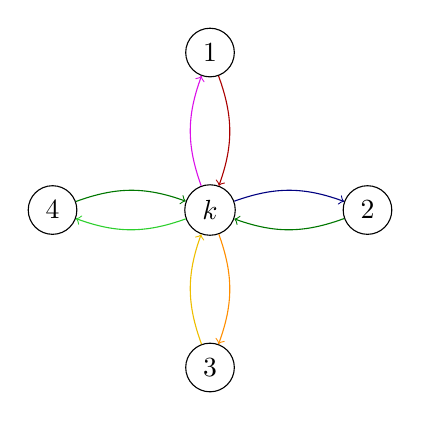
\begin{tikzpicture}
            % Central node
            \node[circle, draw, fill=white, minimum size=0.6cm] (center) at (0,0) {$k$};
        
            % Surrounding nodes
            \node[circle, draw, fill=white, minimum size=0.6cm] (n1) at (0,2) {1};
            \node[circle, draw, fill=white, minimum size=0.6cm] (n2) at (2,0) {2};
            \node[circle, draw, fill=white, minimum size=0.6cm] (n3) at (0,-2) {3};
            \node[circle, draw, fill=white, minimum size=0.6cm] (n4) at (-2,0) {4};
            
            % Arrows
            \draw[->, color=arrow1, bend left=20] (center) to (n1); % Center to 1
            \draw[<-, color=arrow1back, bend right=20] (center) to (n1); % 1 to Center

            \draw[->, color=arrow2, bend left=20] (center) to (n2); % Center to 2
            \draw[<-, color=arrow2back, bend right=20] (center) to (n2); % 2 to Center

            \draw[->, color=arrow3, bend left=20] (center) to (n3); % Center to 3
            \draw[<-, color=arrow3back, bend right=20] (center) to (n3); % 3 to Center

            \draw[->, color=arrow4, bend left=20] (center) to (n4); % Center to 4
            \draw[<-, color=arrow4back, bend right=20] (center) to (n4); % 4 to Center
            
        \end{tikzpicture}
    }
    \caption{Exemplary cutout of a square lattice. The nearest neighbors to a central node with index $k$ are depicted. The numeration is arbitrary, but matches the indices that are used in \autoref{eq:current-geometry-example}.
    The colors match the terms that correspond to their transition.
    }
    \label{fig:current-geometry-example}
\end{SCfigure}

\begin{equation}
    \label{eq:current-geometry-example}
    \begin{split}
        \partial_\text{x}
        j_{\text{x}\,\,k,\,\sigma}^{\,\,\schroedingerPicture}+
        \partial_\text{y} 
        j_{\text{y}\,\,k,\,\sigma}^{\,\,\schroedingerPicture} 
        &\stackrel{\phantom{\ref{eq:continuity-equation}}}{=}
        \textcolor{arrow2}{
            \spinPolarizedKineticsOperatorDir{k}{2}{\sigma}
        }
        -
        \textcolor{arrow4back}{
            \spinPolarizedKineticsOperatorDir{4}{k}{\sigma}
        }\\
        &\stackrel{\phantom{\ref{eq:continuity-equation}}}{+}
        \textcolor{arrow3}{
            \spinPolarizedKineticsOperatorDir{k}{3}{\sigma}
        }
        -
        \textcolor{arrow1back}{
            \spinPolarizedKineticsOperatorDir{1}{k}{\sigma}
        }\\
        & \stackrel{\ref{eq:continuity-equation}}{=}
         - i \cdot \left[\pictureHamiltonian[\schroedingerPicture],\, \nop[\schroedingerPicture]{k}{\sigma}\right]
         \stackrel{\ref{eq:calculation-current-commutator}}{=}\\
         & \hspace{-3cm} i\cdot J \left(
            \textcolor{arrow2}{
                \withspinhcop[\schroedingerPicture]{2}{\sigma}{\dagger}
                \withspinhcop[\schroedingerPicture]{k}{\sigma}{}
            }
            -
            \textcolor{arrow2back}{
                \withspinhcop[\schroedingerPicture]{k}{\sigma}{\dagger}
                \withspinhcop[\schroedingerPicture]{2}{\sigma}{}
            }
            -
            \textcolor{arrow4back}{
                \withspinhcop[\schroedingerPicture]{k}{\sigma}{\dagger}
                \withspinhcop[\schroedingerPicture]{4}{\sigma}{}
            }
            +
            \textcolor{arrow4}{
                \withspinhcop[\schroedingerPicture]{4}{\sigma}{\dagger}
                \withspinhcop[\schroedingerPicture]{k}{\sigma}{}
            }
            +
            \textcolor{arrow3}{
                \withspinhcop[\schroedingerPicture]{3}{\sigma}{\dagger}
                \withspinhcop[\schroedingerPicture]{k}{\sigma}{}
            }
            -
            \textcolor{arrow3back}{
                \withspinhcop[\schroedingerPicture]{k}{\sigma}{\dagger}
                \withspinhcop[\schroedingerPicture]{3}{\sigma}{}
            }
            -
            \textcolor{arrow1back}{
                \withspinhcop[\schroedingerPicture]{k}{\sigma}{\dagger}
                \withspinhcop[\schroedingerPicture]{1}{\sigma}{}
            }
            +
            \textcolor{arrow1}{
                \withspinhcop[\schroedingerPicture]{1}{\sigma}{\dagger}
                \withspinhcop[\schroedingerPicture]{k}{\sigma}{}
            }
         \right)
    \end{split}
\end{equation}


\autoref{eq:spin-polarized-kinetics-operator-definition} describes the resulting observable, that measures such kinetics, depending on the direction \spinPolarizedKineticsOperatorDir{l}{m}{\sigma}.

\begin{equation}
    \label{eq:spin-polarized-kinetics-operator-definition}
    \begin{split}
        \spinPolarizedKineticsOperatorDir{l}{m}{\sigma} &= i J \left(\withspinhcop{m}{\sigma}{\dagger}\withspinhcop{l}{\sigma}{} - \withspinhcop{l}{\sigma}{\dagger}\withspinhcop{m}{\sigma}{}\right)\\
    \end{split}
\end{equation}

In this case, the used basis-states are not eigenstates of the operators. 
$\bracketHelper{N}{\withspinhcop{m}{\sigma}{\dagger}\withspinhcop{l}{\sigma}{}}{K}$ becomes $\delta_{N,\,\vphantom{N}\smash{\tilde{N}}}\cdot n_{m,\,\sigma} \cdot (1-n_{l,\,\sigma} )$, where \ketN[{\vphantom{N}\smash{\tilde{N}}}] is the state obtained when the particle number on site $m,\, \sigma$ and the one of site $l,\, \sigma$ are swapped (this \emph{hopping} only has an effect, when there is a particle on the original site and no particle yet on the target site, or vice versa).
Evaluating the whole operator with the signs correctly and in a efficient manner can best be looked up in the implementation 

\filepath{\cite{selfCode}}{/computation-scripts/observables.py}.

Overall, the evaluation of this observable requires knowing the value of an object of the form presented in \autoref{eq:form-heff-difference}.

\begin{equation}
    \label{eq:form-heff-difference}
    \localObservable{N}{t} =
    i \cdot 
    \left[
        n_{m,\,\sigma} \cdot (1-n_{l,\,\sigma})
        -
        n_{l,\,\sigma} \cdot (1-n_{m,\,\sigma})
    \right]
    \cdot 
    \frac{\psiN[\vphantom{N}\smash{\tilde{N}}]}{\psiN}
    \cdot 
    e^{\HeffOft[\vphantom{N}\smash{\tilde{N}}]-\HeffOft[N]}
\end{equation}

The \fullref{sec:theory-optimizations-analytical} will go into how to compute this efficiently for states \ketN[N] and \ketN[{\vphantom{N}\smash{\tilde{N}}}] that are connected via the hopping between nearest-neighbor lattice sites.

It is finally important to notice, that the objects from \autoref{eq:form-heff-difference} are not real-valued, but complex.
Only the complete observable with the full sum over all basis-states \ketN over \localObservable{N}{t} has a fully vanishing imaginary part. 
Especially when the observable is approximated with an incomplete set of basis-states, computationally an imaginary component remains. 
It is important to monitor the magnitude of this value and monitor it going to $0$.
If it doesn't fully vanish, this indicates an error in the sampling strategy or the implementation or the number of sampled states is not great enough.

One could entertain the question, whether is is guaranteed for the imaginary part to vanish with a large enough sample size.
On first thought, if the hamiltonian is only approximated, might there be a possibility for asymmetrical terms to introduce a non-vanishing imaginary part?

Conveniently, rewriting \autoref{eq:expectation-value} in the manner of \autoref{eq:imaginary-part-vanishes}, yields two expressions for the value of the observation that are complex conjugations of each other.
This again means, that no matter how \glqq bad\grqq{} the \psiOfT[\schroedingerPicture] approximates the real wave-function, for full sampling the result must have an imaginary part of 0.

\begin{equation}
    \label{eq:imaginary-part-vanishes}
    \begin{split}
        \frac{\bracketHelper{\psiOfT[\schroedingerPicture]}{\ObservableOp}{\psiOfT[\schroedingerPicture]}}{\braketHelper{\psiOfT[\schroedingerPicture]}{\psiOfT[\schroedingerPicture]}}
        &\cdot
        \left(
            \lsum[K] \absSquare{e^{\HeffOft[K]}} \absSquare{\psiN[K]} 
        \right) =\\
        %
        \lsum[N]
        \absSquare{e^{\HeffOft}} \absSquare{\psiN} 
        \frac{\bracketHelper{N}{\ObservableOp}{\psiOfT[\schroedingerPicture]}}{\braketHelper{N}{\psiOfT[\schroedingerPicture]}}
        &\stackrel{\ast}{=}
        \lsum[N]
        \absSquare{e^{\HeffOft}} \absSquare{\psiN} 
        \frac{\bracketHelper{\psiOfT[\schroedingerPicture]}{\ObservableOp}{N}}{\braketHelper{\psiOfT[\schroedingerPicture]}{N}}
    \end{split}
\end{equation}